\documentclass[twocolumn,natbib]{svjour3}          % twocolumn


\smartqed  % flush right qed marks, e.g. at end of proof
\usepackage{balance}
\balance
\usepackage{dblfloatfix}
\usepackage{placeins}
\usepackage{float}
\usepackage[utf8]{inputenc}
\usepackage{graphicx}
\usepackage{amssymb}
\usepackage{ upgreek }
\usepackage{hyperref}
\usepackage{amsmath}
\usepackage{multirow}
\usepackage[table,xcdraw]{xcolor}
\usepackage{booktabs}
\usepackage{subcaption}
\usepackage[acronym]{glossaries}
\usepackage{breakurl} 
\usepackage{amsmath}
\usepackage{appendix}
\usepackage{verbatim}
\usepackage{listings}
\usepackage{hhline}
\usepackage{tikz}

\newcommand{\tikzmark}[1]{\tikz[remember picture,overlay, baseline=-0.5ex]\node (#1){};}
\newcommand{\connect}[3][3mm]{\tikz[remember picture,overlay]\draw[red,dashed,shorten <=-#1, shorten >=-#1](#2)--(#3);}


\sloppy
\newcounter{constraint}
\newcommand{\nextconstraint}{\refstepcounter{constraint}\arabic{constraint}.}


\title{Disruptions in Timetables:  \large  A Case Study  at Universidade de Lisboa\thanks{This work was supported by Universidade de Lisboa, Instituto Superior T\'ecnico and Departamento de Engenharia Inform\'atica (DEI) and by national funds through Funda\c{c}\~ao para a Ci\^encia e a Tecnologia (FCT) with reference SFRH/BSAB/143643/2019 (sabbatical grant) and UID/CEC/50021/2019 (INESC-ID multi-annual funding).} }
\titlerunning{Disruptions in Timetables at Universidade de Lisboa} 
\author{Alexandre Lemos \and 
Pedro T. Monteiro \and  Inês Lynce}
%

% First names are abbreviated in the running head.
% If there are more than two authors, 'et al.' is used.
%
\institute{A. Lemos \and P.T. Monteiro \and I. Lynce  \at Instituto Superior T\'ecnico, Universidade de Lisboa\\ INESC-ID,
Rua Alves Redol, 9, 1000-029 Lisboa, Portugal\\
\email{\{alexandre.lemos,pedro.tiago.monteiro,ines.lynce\}\\@tecnico.ulisboa.pt}
}
%
\newcommand{\uni}{\gls{ist}}
\date{Received: date / Accepted: date}
\journalname{Journal of Scheduling}
\begin{document}



\maketitle  
\begin{abstract}
Solving university timetabling problems is a large and complex task. Moreover, every new academic year, a new timetable is likely to be scheduled due to minor disruptions. However, a timetable does not need to be periodically scheduled from scratch since it can produce a completely different solution from the previous one, thus creating undesirable changes for many actors.

This paper addresses the \gls{mpp} in university timetabling. Given a set of disruptions that make a timetable no longer feasible, a solution to the \gls{mpp} is the \textit{closest} new feasible timetable with respect to the original timetable. We propose and analyze two different integer programming models to encode the \gls{mpp}. To validate the proposed models, disruptions are randomly generated based on the probability distributions learned from the history of timetables over the last five years in the \uni \ the engineering school from Universidade de Lisboa. Overall, our models, combined with an incremental approach, are shown to be able to efficiently solve all problem instances.

  \keywords{Minimal Perturbation Problem \and University Timetabling \and Disruption \and Integer Programming.}
  
\end{abstract}


\section{Introduction}

\begin{figure*}[t]
	
	
	\renewcommand{\arraystretch}{2}
	\newcolumntype{P}[1]{>{\centering\arraybackslash}p{#1}}
	\begin{subfigure}{.5\textwidth}
		\centering
		\resizebox{\textwidth}{!}{%
			\begin{tabular}{|c||cc|P{1.4cm}|P{1.4cm}|P{1.4cm}|P{1.4cm}|p{.2cm}}
				\cline{1-7}
				\textbf{}        & \multicolumn{2}{c|}{\textbf{Mon} }                                  & \textbf{Tue}                                  & \textbf{Wed}                                  & \textbf{Thu}                                      & \textbf{Fri}                                              &               \\ \hhline{*7-}\morecmidrules \hhline{*7-}
				\textbf{8:00}    &     \multicolumn{2}{c|}{}                                           &                                               & \cellcolor[HTML]{5379FA}                      &                                                   &                                                           & \\  \hhline{*4{>{\arrayrulecolor{black}}-}*1{>{\arrayrulecolor[HTML]{5379FA}}-}*2{>{\arrayrulecolor{black}}-}} 
				\textbf{8:30}    &     \multicolumn{2}{c|}{}                                           &                                               & \cellcolor[HTML]{5379FA} B\textsuperscript{PB}&                                                   &                                                           & \\ \hhline{*4{>{\arrayrulecolor{black}}-}*1{>{\arrayrulecolor[HTML]{5379FA}}-}*2{>{\arrayrulecolor{black}}-}}
				\textbf{9:00}    & \multicolumn{2}{c|}{ \cellcolor[HTML]{FEFFCF}}                      &                                               & \cellcolor[HTML]{5379FA} (R2)                 & \cellcolor[HTML]{FEFFCF}                          &   \cellcolor[HTML]{FEFFCF}                                &  \\ \hhline{*1{>{\arrayrulecolor{black}}-}*2{>{\arrayrulecolor[HTML]{FEFFCF}}-}*2{>{\arrayrulecolor{black}}-}*2{>{\arrayrulecolor[HTML]{FEFFCF}}-}}\arrayrulecolor{black}
				\textbf{9:30}    & \multicolumn{2}{c|}{\cellcolor[HTML]{FEFFCF} A\textsuperscript{T}}  &                                               & \cellcolor[HTML]{FEFFCF}                      & \cellcolor[HTML]{FEFFCF} A\textsuperscript{T}     &     \cellcolor[HTML]{FEFFCF} B\textsuperscript{T}         & \\ \hhline{*1{>{\arrayrulecolor{black}}-}*2{>{\arrayrulecolor[HTML]{FEFFCF}}-}*1{>{\arrayrulecolor{black}}-}*3{>{\arrayrulecolor[HTML]{FEFFCF}}-}}\arrayrulecolor{black}
				\textbf{10:00}   & \multicolumn{2}{c|}{\cellcolor[HTML]{FEFFCF}    (R1)}               &                                               & \cellcolor[HTML]{FEFFCF} B\textsuperscript{T} &  \cellcolor[HTML]{FEFFCF} (R1)                    & \cellcolor[HTML]{FEFFCF}    (R1)                          &   \\ \hhline{*4{>{\arrayrulecolor{black}}-}*1{>{\arrayrulecolor[HTML]{FEFFCF}}-}*2{>{\arrayrulecolor{black}}-}}
				\textbf{10:30}   &  \multicolumn{1}{c|}{\cellcolor[HTML]{E68680} }                      &\tikzmark{p1} \hspace{.8cm} \cellcolor[HTML]{CFCFE7}  \tikzmark{p2}                    & & \cellcolor[HTML]{FEFFCF}   (R1)             &\cellcolor[HTML]{5379FA}                           &    \cellcolor[HTML]{FEFFCF} C\textsuperscript{T}                                &  \\ \hhline{*1{>{\arrayrulecolor{black}}-}*1{>{\arrayrulecolor[HTML]{E68680}}-}*1{>{\arrayrulecolor[HTML]{CFCFE7}}-}*2{>{\arrayrulecolor{black}}-}*1{>{\arrayrulecolor[HTML]{5379FA}}-}*1{>{\arrayrulecolor[HTML]{FEFFCF}}-}} \arrayrulecolor{black}
				\textbf{11:00}   &  \multicolumn{1}{c|}{\cellcolor[HTML]{E68680} A\textsuperscript{L} } & \cellcolor[HTML]{CFCFE7} A\textsuperscript{L} &                                               & \cellcolor[HTML]{FEFFCF} D\textsuperscript{T}     &   \cellcolor[HTML]{5379FA} D\textsuperscript{PB} &  \cellcolor[HTML]{FEFFCF}    (R1)                &  \\ \hhline{*1{>{\arrayrulecolor{black}}-}*1{>{\arrayrulecolor[HTML]{E68680}}-}*1{>{\arrayrulecolor[HTML]{CFCFE7}}-}*1{>{\arrayrulecolor{black}}-}*1{>{\arrayrulecolor[HTML]{FEFFCF}}-}*1{>{\arrayrulecolor[HTML]{5379FA}}-}*1{>{\arrayrulecolor{black}}-}} \arrayrulecolor{black}
				\textbf{11:30}   &  \multicolumn{1}{c|}{\cellcolor[HTML]{E68680}(R4)}  & \tikzmark{p3} \cellcolor[HTML]{CFCFE7}  (R3) \tikzmark{p4}          &                                               & \cellcolor[HTML]{FEFFCF}  (R1)                    & \cellcolor[HTML]{5379FA}    (R2)   &   \cellcolor[HTML]{FEFFCF}   D\textsuperscript{T}                                  &   \\ \hhline{*6{>{\arrayrulecolor{black}}-}*1{>{\arrayrulecolor[HTML]{FEFFCF}}-}} \arrayrulecolor{black}
				\textbf{12:00}   &\multicolumn{2}{c|}{\cellcolor[HTML]{FEFFCF}   C\textsuperscript{T}} &                                               & \cellcolor[HTML]{FEFFCF} C\textsuperscript{T} &\cellcolor[HTML]{5379FA}                           &  \cellcolor[HTML]{FEFFCF} (R1)      &     \\ \hhline{*1{>{\arrayrulecolor{black}}-}*2{>{\arrayrulecolor[HTML]{FEFFCF}}-}*1{>{\arrayrulecolor{black}}-}*1{>{\arrayrulecolor[HTML]{FEFFCF}}-}*1{>{\arrayrulecolor[HTML]{5379FA}}-}*1{>{\arrayrulecolor{black}}-}} \arrayrulecolor{black}
				\textbf{12:30}   &\multicolumn{2}{c|}{\cellcolor[HTML]{FEFFCF} (R1)}                   &  \cellcolor[HTML]{5379FA}                     & \cellcolor[HTML]{FEFFCF} (R1)                 &   \cellcolor[HTML]{5379FA}D\textsuperscript{PB}   &  \cellcolor[HTML]{5379FA}                                                 &       \\ \hhline{*3{>{\arrayrulecolor{black}}-}*1{>{\arrayrulecolor[HTML]{5379FA}}-}*1{>{\arrayrulecolor{black}}-}*2{>{\arrayrulecolor[HTML]{5379FA}}-}} \arrayrulecolor{black}
				\textbf{13:00}   & \multicolumn{2}{c|}{\cellcolor[HTML]{FEFFCF} D\textsuperscript{T} } & \cellcolor[HTML]{5379FA} C\textsuperscript{PB}&                                               &\cellcolor[HTML]{5379FA}    (R2)                   & \cellcolor[HTML]{5379FA}   B\textsuperscript{PB}    &                                                 \\ \hhline{*1{>{\arrayrulecolor{black}}-}*2{>{\arrayrulecolor[HTML]{FEFFCF}}-}*1{>{\arrayrulecolor[HTML]{5379FA}}-}*2{>{\arrayrulecolor{black}}-}*1{>{\arrayrulecolor[HTML]{5379FA}}-}} \arrayrulecolor{black}
				\textbf{13:30}   &\multicolumn{2}{c|}{\cellcolor[HTML]{FEFFCF}  (R1)}                  & \cellcolor[HTML]{5379FA}   (R2)               &                                               &                                                   &  \cellcolor[HTML]{5379FA} (R2)                                        & \\ \cline{1-7}
				
		\end{tabular}	\connect{p1}{p4}
\connect{p2}{p3}}
	
		\caption{Before}
		\label{fig:before}
	\end{subfigure}%
	\begin{subfigure}{.5\textwidth}
		\centering
		\resizebox{.94\textwidth}{!}{%
			\begin{tabular}{|c||P{1.4cm}|P{1.4cm}|P{1.4cm}|P{1.4cm}|P{1.4cm}|p{0.4cm}}
				\cline{1-6}
				\textbf{}        & \textbf{Mon}                                         & \textbf{Tue}                                      & \textbf{Wed}                                          & \textbf{Thu}                                      & \textbf{Fri}                                          &               \\ \hhline{*6-}\morecmidrules \hhline{*6-}
				\textbf{8:00}    &                                                      &                                                   &   \cellcolor[HTML]{5379FA}                            &                                                   &                                                       &   \\ \hhline{*3{>{\arrayrulecolor{black}}-}*1{>{\arrayrulecolor[HTML]{5379FA}}-}*2{>{\arrayrulecolor{black}}-}}\arrayrulecolor{black}
				\textbf{8:30}    &                                                      &                                                   &  \cellcolor[HTML]{5379FA}  B\textsuperscript{PB}      &                                                   &                                                       &  \\\hhline{*3{>{\arrayrulecolor{black}}-}*1{>{\arrayrulecolor[HTML]{5379FA}}-}*2{>{\arrayrulecolor{black}}-}}\arrayrulecolor{black}
				\textbf{9:00}    &  \cellcolor[HTML]{FEFFCF}                            &                                                   &  \cellcolor[HTML]{5379FA}   (R2)                      &  \cellcolor[HTML]{FEFFCF}                         &\cellcolor[HTML]{FEFFCF}                               & \\ \hhline{*1{>{\arrayrulecolor{black}}-}*1{>{\arrayrulecolor[HTML]{FEFFCF}}-}*2{>{\arrayrulecolor{black}}-}*2{>{\arrayrulecolor[HTML]{FEFFCF}}-}}\arrayrulecolor{black}
				\textbf{9:30}    & \cellcolor[HTML]{FEFFCF} A\textsuperscript{T}        &                                                   &   \cellcolor[HTML]{FEFFCF}                            &   \cellcolor[HTML]{FEFFCF} A\textsuperscript{T}   &     \cellcolor[HTML]{FEFFCF}  B\textsuperscript{T}    &  \\ \hhline{*1{>{\arrayrulecolor{black}}-}*1{>{\arrayrulecolor[HTML]{FEFFCF}}-}*1{>{\arrayrulecolor{black}}-}*3{>{\arrayrulecolor[HTML]{FEFFCF}}-}}\arrayrulecolor{black}
				\textbf{10:00}   & \cellcolor[HTML]{FEFFCF}  (R1)                       &                                                   &   \cellcolor[HTML]{FEFFCF} B\textsuperscript{T}       &  \cellcolor[HTML]{FEFFCF} (R1)                    &    \cellcolor[HTML]{FEFFCF}  (R1)                     &    \\ \hhline{*3{>{\arrayrulecolor{black}}-}*1{>{\arrayrulecolor[HTML]{FEFFCF}}-}*2{>{\arrayrulecolor{black}}-}}\arrayrulecolor{black}
				\textbf{10:30}   & \cellcolor[HTML]{E68680}                             &   \cellcolor[HTML]{E68680}                         & \cellcolor[HTML]{FEFFCF}  (R1)                        &\cellcolor[HTML]{5379FA}                           &    \cellcolor[HTML]{FEFFCF}    C\textsuperscript{T}   &   \\ \hhline{*1{>{\arrayrulecolor{black}}-}*2{>{\arrayrulecolor[HTML]{E68680}}-}*1{>{\arrayrulecolor{black}}-}*1{>{\arrayrulecolor[HTML]{5379FA}}-}*1{>{\arrayrulecolor[HTML]{FEFFCF}}-}}\arrayrulecolor{black}
				\textbf{11:00}   & \cellcolor[HTML]{E68680} A\textsuperscript{L}        & \cellcolor[HTML]{E68680} A\textsuperscript{L}     & \cellcolor[HTML]{FEFFCF}   D\textsuperscript{T}       &   \cellcolor[HTML]{5379FA} D\textsuperscript{PB}  &  \cellcolor[HTML]{FEFFCF}       (R1)                  &         \\ \hhline{*1{>{\arrayrulecolor{black}}-}*2{>{\arrayrulecolor[HTML]{E68680}}-}*1{>{\arrayrulecolor[HTML]{FEFFCF}}-}*1{>{\arrayrulecolor[HTML]{5379FA}}-}*1{>{\arrayrulecolor{black}}-}}\arrayrulecolor{black}
				\textbf{11:30}   & \cellcolor[HTML]{E68680} (R4)                        & \cellcolor[HTML]{E68680} (R4)                     & \cellcolor[HTML]{FEFFCF}  (R1)                        & \cellcolor[HTML]{5379FA}    (R2)                  &   \cellcolor[HTML]{FEFFCF}     D\textsuperscript{T}   &  \\ \hhline{*5{>{\arrayrulecolor{black}}-}*1{>{\arrayrulecolor[HTML]{FEFFCF}}-}}\arrayrulecolor{black}
				\textbf{12:00}   &\cellcolor[HTML]{FEFFCF}  C\textsuperscript{T}        &                                                   & \cellcolor[HTML]{FEFFCF}   C\textsuperscript{T}       &\cellcolor[HTML]{5379FA}                           &  \cellcolor[HTML]{FEFFCF} (R1)                        &      \\ \hhline{*1{>{\arrayrulecolor{black}}-}*1{>{\arrayrulecolor[HTML]{FEFFCF}}-}*1{>{\arrayrulecolor{black}}-}*1{>{\arrayrulecolor[HTML]{FEFFCF}}-}*1{>{\arrayrulecolor[HTML]{5379FA}}-}*1{>{\arrayrulecolor{black}}-}}\arrayrulecolor{black}  
				\textbf{12:30}   &\cellcolor[HTML]{FEFFCF}  (R1)                        &  \cellcolor[HTML]{5379FA}                     &   \cellcolor[HTML]{FEFFCF}  (R1)                      &   \cellcolor[HTML]{5379FA} D\textsuperscript{PB}  &  \cellcolor[HTML]{5379FA}                             &    \\ \hhline{*2{>{\arrayrulecolor{black}}-}*1{>{\arrayrulecolor[HTML]{5379FA}}-}*1{>{\arrayrulecolor{black}}-}*2{>{\arrayrulecolor[HTML]{5379FA}}-}}\arrayrulecolor{black}
				\textbf{13:00}   & \cellcolor[HTML]{FEFFCF}  D\textsuperscript{T}       & \cellcolor[HTML]{5379FA}  C\textsuperscript{PB}   &                                                       &\cellcolor[HTML]{5379FA}    (R2)                   & \cellcolor[HTML]{5379FA}   B\textsuperscript{PB}      &    \\ \hhline{*1{>{\arrayrulecolor{black}}-}*1{>{\arrayrulecolor[HTML]{FEFFCF}}-}*1{>{\arrayrulecolor[HTML]{5379FA}}-}*2{>{\arrayrulecolor{black}}-}*1{>{\arrayrulecolor[HTML]{5379FA}}-}}\arrayrulecolor{black}
				\textbf{13:30}   & \cellcolor[HTML]{FEFFCF}  (R1)                       & \cellcolor[HTML]{5379FA}  (R2)                    &                                                       &                                                   &  \cellcolor[HTML]{5379FA}  (R2)                       &   \\ \cline{1-6}
		\end{tabular}}
		\caption{After}
		\label{fig:after}
	\end{subfigure}
	\caption{Timetable for a class of students (a) before and (b) after occurring two disruptions: (i) an  \textit{unavailability} constraint over room R3 and (ii) a \textit{no overlap} constraint \textit{w.r.t.} the two lab lectures of course A. The colors represent the different rooms the lectures are assigned to.}
	\label{fig:original}
\end{figure*}


%The aim of the paper and the reason why
University timetabling problems in real-world scenarios are one of the major open challenges in university timetabling problems~\citep{mccollum2006university,DBLP:journals/anor/VrielinkJHH19}. Given a set of constraints a solution to a university timetabling problem is an assignment to all lectures to suitable rooms and time slots in such a way that all the constraints  are satisfied. University timetabling problems are known to be NP-complete~\citep{DBLP:journals/siamcomp/EvenIS76} given that the search space for possible solutions grows exponentially with the number of lectures. 

%A bit more motivation about reformulation
Every semester a new timetable needs to be created. Usually, the number of changes between the timetables of consecutive years is small. These changes can be of different types: either constraints are added/changed, or the domain of a variable is changed. These changes may cause the original solution to be infeasible. Solving the problem from scratch may negatively affect many of the actors involved. However, it is not necessary to generate a completely new timetable each semester. This problem can be considered a \acrlong{mpp} where the existing solution is no longer feasible and one needs to find the \textit{closest} feasible solution. 

\paragraph{MPP}
Given a set of disruptions and a timetable, a solution to a \acrlong{mpp} is a solution to a university timetabling problem while minimizing a distance function $\delta$, which  computes the distance between the original solution and the new feasible solution.

%Case study and motivation from the case study
Solving the \gls{mpp} instead of solving the problem from scratch can improve user satisfaction with the resulting timetable. Actually, this is the approach taken by the academic services at \gls{ist}. Most often, the disruptions result from changes in teacher-lecture allocation, curricular plans and number of students. In addition, when specific problems referring to previous timetables are reported, one can learn from previous mistakes. Besides these changes, the academic services assume that everything else in the timetable is acceptable. For this reason, and if possible, those parts of the timetable will continue unchanged. This assumption allows the services to reduce the scope of the problem. 

%Small note
In the context of university timetabling, there is one more scenario that is considered an \gls{mpp}. The university is a dynamical system and thus the timetables should be able to change even during their execution.  







\begin{example}\label{ex:mov}
	Let us consider the timetable shown in Figure~\ref{fig:before}. The weekly timetable shows the different lectures of the different courses a student can attend. Each student having this curricular plan must attend some lectures from the four courses represented (A to D). For each course, a student must attend all theoretical lectures and only one practical / laboratory lecture. For example, a student must attend all A\textsuperscript{T} (theoretical) lectures in the schedule and only one of the two A\textsuperscript{L} (laboratory) possible lectures. 
	
	
	Consider the following disruptions applied to the given example: (i) room R3 is closed for renovations for a long period of time and (ii) the number of teachers available to teach A\textsuperscript{L} is now only one. Consider that we want to cause the smallest number of perturbations ($\delta$) to the original solution. Disruption (i) reduces the domain of the problem. In this small example, one lecture is assigned to R3. Therefore, the original solution (\ref{fig:before}) is no longer feasible. If one considers that there are only two laboratories (R4 and R3), and that R4 is already taken in the required time slot, then we conclude that the optimal solution requires two perturbations to the original solution (change room and time). Disruption (ii) adds a new {\em no overlap} constraint to the model. Note, however, that any solution containing the perturbations resulting from the first disruption already works out for this disruption. A possible solution is shown in Figure~\ref{fig:after}.
\end{example}


%Contributions
The contribution of this paper is two-fold: (i) two different integer programming models (\textsc{Boolean} and \textsc{mixed}) to encode the \gls{mpp} applied to university timetabling, and (ii) an incremental algorithm to solve these models efficiently.
We showcase the application of the models in real-world problem instances using data sets from \uni. The disruptions are generated with different probabilities to match the history of disruptions of the case study.

%Organization
This paper is organized as follows. Section~\ref{sec:rel} provides a brief overview of the relevant state of the art. Section~\ref{sec:pro} formally describes the problem. Section~\ref{sec:model} describes the different models to encode the problem.  Section~\ref{sec:eval}  discusses the generation of disruptions based on history and shows the computational results for the different models and disruptions. Finally, Section~\ref{sec:con} concludes the paper and addresses future work.



\section{Related Work}\label{sec:rel}
\subsection{Timetables}
University timetabling problems~\citep{DBLP:series/sci/Kingston13,mccollum2006university,DBLP:journals/anor/VrielinkJHH19}  can be classified into two major categories: examination timetabling~\citep{M2009} and course timetabling problems~\citep{di2007second}. Many different approaches have been successfully applied for solving these problems, namely  \gls{cp}~\citep{DBLP:conf/patat/MullerRB04}, \gls{asp}~\citep{DBLP:journals/anor/BanbaraIKOSSTW19}, Boolean Satisfiability~(SAT)~\citep{DBLP:journals/anor/AchaN14}, \gls{ilp}~\citep{LEMOS2018100092,LINDAHL2019,DBLP:conf/wea/LachL08,DBLP:journals/eor/VermuytenLMB16,DBLP:journals/cor/CacchianiCRT13}, genetic algorithms~\citep{DBLP:journals/anor/PillayO19} and local search~\citep{LEMOS2018100092,DBLP:conf/patat/grasp,DBLP:journals/scheduling/BellioGS12}.

In recent years, a siginificant improvement in solving course timetabling problems have been achieved~\citep{Bettinelli2015}. Behind this progress lies the public data sets from ITC~\citep{di2007second}, which are a simplified version of the real timetabling problem at the University of Udine. For this reason, the progress made still presents a gap between theory and practice~\citep{mccollum2006university} since it does not capture the full complexity of the real world problem.

\cite{DBLP:journals/eor/VermuytenLMB16} proposed a two-stage approach to optimize student flows using \gls{ilp}. The methods were tested using the real data of \gls{kul}. The \gls{kul} data is more complex than the simplified ITC data. However, it also adds specific problems that are inherent to the \gls{kul} data.


\cite{LEMOS2018100092} proposed three different approaches to optimize space usage in university timetabling while ensuring the maximum number of students are able to attend their lectures. Two of these approaches solve the problem using greedy heuristics which are able to solve efficiently the problem. Nevertheless, they fall short of the optimal value. Therefore, the authors proposed an \gls{ilp} approach which is slower but it is able to find the optimal solution for every instance tested. All aproaches were tested using a very large data set corresponding to the data from \uni. The work proposed in this paper is an extension to our previous work~\citep{LEMOS2018100092} in order to solve \gls{mpp}.  %The results for the greedy heuristics are not shown here since they are worse in terms of quality and similar in terms of CPU time.
  

\subsection{Minimal Perturbation Problem}

Given a solution to a problem instance and a set of disruptions which make the solution no longer feasible, solving the \gls{mpp} is the task of finding a new feasible solution requiring the smallest number of perturbations \citep{DBLP:journals/constraints/SakkoutW00,DBLP:journals/constraints/ZivanGM11,APhillips2017}. 
The \gls{mpp} adds an optimization criterion to the course  timetabling problem. The goal of this criterion is to evaluate the distance between the solutions, \emph{i.e.} the number of perturbations required to go from one solution to another (formally defined in Section 3). The most commom approach \citep{DBLP:journals/constraints/ZivanGM11,APhillips2017,DBLP:conf/patat/MullerRB04,DBLP:journals/anor/BanbaraIKOSSTW19,LINDAHL2019} is to apply the Hamming Distance~\citep{6772729}. However, this metric lacks domain knowledge.



\cite{DBLP:conf/patat/MullerRB04} proposed the iterative forward search algorithm to solve the \gls{mpp} applied to university timetabling. Since this method is a local search method, it does not ensure completeness. \cite{APhillips2017} use integer programming to solve \gls{mpp} on instances from the University of Auckland. The proposed method tries to solve the problem in the smallest possible neighborhood. If feasible solution is not found, then the neighborhood is gradually expanded until either a feasible solution is found or the neighborhood includes the whole search space. 

\cite{DBLP:journals/anor/BanbaraIKOSSTW19} proposed an \gls{asp} based tool to compute Pareto fronts with two objectives: (i) minimize the number of soft constraints unsatisfied and (ii) minimize the number of perturbations. The tool solves the \gls{mpp} if and only if the disruption changes the course  timetabling problem by adding or removing constraints. Therefore, all disruptions that cause the domain of the problem to change cannot be solved by this tool. 

Recently, \cite{LINDAHL2019} proposed a bi-objective integer programming model to solve \gls{mpp} applied to curriculum-based course timetabling. The goal is to find Pareto-optimal solutions for these two objectives: (i) minimize the number of perturbations and (ii) minimize the number of soft constraints unsatisfied. The results show that the \gls{mpp} solutions often have low quality and that allowing few more perturbations can significantly improve the quality. \cite{LINDAHL2019} approach evaluated with data sets from the 2007 \gls{itc}. 

\subsection{Disruptions in University Timetabling}



\begin{table*}[!h]
	\renewcommand{\arraystretch}{1.5}
	\centering
	\caption{Summary and literature review of the most common disruptions in a university scenario. The implications in problem structure are classified as changes in the domain~($\mathcal{D}$) of the sets or changes in the set of constraints~($\mathcal{C}$).}
	\label{tab:perturbations}
	\resizebox{\textwidth}{!}{%
		\begin{tabular}{|l|c|c|c|c|c|c|}
			\hline 
			
			\multicolumn{1}{|c|}{Disruption}                      & \cite{LINDAHL2019}      & \cite{APhillips2017}     & \cite{DBLP:conf/patat/MullerRB04} & \cite{DBLP:journals/anor/BanbaraIKOSSTW19}      & Other & \multicolumn{1}{c|}{Cause}         \\  \hline \hline
			Room Stability       &  &                             & & $\checkmark$ & & $\mathcal{C}$     \\ \hline
			Overlap/No Overlap      &  &              &               & & $\checkmark$ & $\mathcal{C}$      \\ \hline
			Invalid Assignment      & $\checkmark$ &              & $\checkmark$ & & &$\mathcal{C}$  \\ \hline
			Invalid/Preference Time &   $\checkmark$ & $\checkmark$ &              & & &$\mathcal{C}$  \\ \hline
			Invalid/Preference Room    &  & &              & & $\checkmark$ & $\mathcal{C}$ \\ \hline
			Remove Room for a day   & $\checkmark$ &              &              & & &$\mathcal{C}$ \\ \hline
			Remove Room    &  & $\checkmark$             &             &  &  &   $\mathcal{D}$             \\ \hline
			Insert Curriculum       & $\checkmark$ &              &              & & &$\mathcal{D}$     \\ \hline
			Modify Enrollments     &             & $\checkmark$ &              & & &$\mathcal{D}$  \\ \hline  
			Modify \# Lectures       &  &              &               & & $\checkmark$ & $\mathcal{D}$     \\ \hline
			
			
	\end{tabular}}
\end{table*}



There are different types of disruptions which can be categorized as follows: changes in the domain~($\mathcal{D}$) of the sets (\emph{e.g.} remove a room) or a change in the set of constraints~($\mathcal{C}$) (\emph{e.g.} remove a room for a day). Table~\ref{tab:perturbations} summarizes the different disruptions that can occur in university timetabling.  The most common disruptions that can occur when re-solving university timetabling problems are following:

\begin{itemize}
\item {\it Room stability}: disruption forces all lectures of a course to be scheduled in the same room.
\item {\it Overlap} ({\it no overlap}): disruption refers to the addition of a constraint to forbid (force) lectures to be taught simultaneously. For example, {\it no overlap} disruption may arise when the number of teachers assigned to a course reduces to one.
\item  {\it Invalid assignment}: disruption refers to a problem in the assignment of the lecture to a room or to a time slot. This disruption abstracts the origin of the problem (time or room assignment). However, in a real-world scenario it is more common to find more specific disruptions.  
\item {\it Invalid time} and {\it invalid room}: are disruptions that make an assignment of a lecture to a time slot and a room invalid, respectively. These two last disruptions are more specific than the {\it invalid assignment} disruption. Note that, these disruptions can be further specified when only a time slot or a room is unavailable to only a specific set of courses. {\it Preference time} and {\it room preference} are the opposite disruptions of the {\it invalid time } and {\it invalid room}.
\item {\it Remove room for a day} and {\it remove room}: cause a room unavailability for an assignment for a day and forever, respectively.
\item  {\it Insert curriculum}: adds a new set of courses. Each lecture of the new courses cannot be overlapped in time. All constraints relating to lectures are applied (\emph{e.g.} room capacity).
\item {\it Modify enrollments}: modifies the number of students that are enrolled in a lecture, since it naturally between the execution of consecutive years. The disruption may not require changes in the original solution since the difference may still be supported.  
\item {\it Modify Number of Lectures}: adds/removes the number of possible lectures that a student can attend. The number of lectures does not change for each student. However, the students have more/less flexibility in their choice of timetable. This disruption can be a side effect of the {\it modify enrollments} disruption.
\end{itemize}
    



The model proposed by \cite{LINDAHL2019}  only considered the following disruptions: \textit{remove room for a day}, \textit{invalid time}, \textit{insert curriculum}, and \textit{invalid assignment}.
With these set of disruptions, one can define an upper bound on the number of satisfied soft constraints since they cannot improve the quality of the original solution. The disruptions reduce the search space. However, in this work, we consider different types of disruptions, such as disruptions that change the problem variable's domain and may lead to a solution with better quality. Therefore, we cannot simply apply the algorithm proposed by \cite{LINDAHL2019} as shown in Example 2.

\begin{example}
	Let us consider that the lecture C\textsuperscript{T}, shown in Figure~\ref{fig:before}, has 125 students enrolled. Room R1 has a capacity of only 110 students. Consider that R1 is the only room with enough capacity to fit more than 100 students. When generating the new timetable (based on the last semester), a disruption causes the number of students enrolled in C\textsuperscript{T} to be reduced to only 105. This disruption causes the overall quality of the timetable to improve.
\end{example}





\section{Problem Definition}\label{sec:pro}


In this section we formally introduce the problem and the notation used throughout the text.

\subsection{Preliminaries}

Let us consider a set of periods $P \in \{0,...,120\}$ corresponding to all possible time slots of a working week ($|P| = |D| \times |T|$). These periods are separated in working days $D \in \{0,...,4\}$ (0 corresponding to Monday, 1 to Tuesday, and so on). Each day has a set of consecutive working time slots of half an hour, $T \in \{0,...,23\}$\footnote{We consider that the rooms are available for use only between $8$am and $8$pm, corresponding to a total of $12$ hours and 24 slots of half an hour.}. The university has a set $R$ of rooms where lectures can be scheduled. All university lectures $L$ (from different courses) have to be assigned to a time slot and to a room. 

Consider a set of courses $C$, with each course $c \in C$ having a set of lectures $\mathcal{L}_c$ in which a set of students ($S$) can be enrolled in. Each set $\mathcal{L}_c$ is composed by $n$ disjoint subsets of lectures ($L_c^{1, \ldots, n} \subseteq \mathcal{L}_c$) of different types (\emph{e.g. }theoretical, practical, laboratory). A student enrolled in course $c$ must attend exactly one lecture of each set $L_c^{i}$. Each subset of lectures $L_c^i \subseteq \mathcal{L}_c$, where $1\leq i \leq n$, has a value $overlap_{L_c^{i}}$ associated, with $0 < overlap_{L_c^{i}} \leq |L_c^{i}|$, where $overlap_{L_c^{i}}$ represents the number of lectures of $L_c^{i}$ that can be overlapped. In other words, $overlap_{L_c^{i}}$  represents the smallest number of teachers\footnote{The assignment of teachers to lectures is only performed after the schedule is created. Therefore, this number is computed based on the timetables from the previous year.\vspace{.5cm}} in charge of lectures in $L_c^i$. 

Furthermore, a lecture $l \in L$ is characterized by: a set of enrolled students ($S_l \subseteq S$) of size $std_l$; a set of suitable rooms ($R_l \subseteq R$);
a set of suitable days  ($D_l \subseteq D$);
a set of suitable  time slots ($T_l \subseteq T$);
and its duration ($len_l > 1$).

Each student $s \in S$ has a set of lectures $L_s \subseteq L$ where he is enrolled in. Since all weeks have basically the same lectures, one can generate the timetables for one week and generalize for the weeks of the whole semester.


Finally, each lecture has to be assigned to a suitable room ($R_l$). Each room $r$, with $r \in R$, has an ideal capacity, $cap_r > 0$. To ensure a fair distribution for students, we add a slack variable of $\alpha$, representing the percentage of students enrolled in a lecture for which it is acceptable to be over the ideal capacity of the assigned room (\emph{i.e.} overbooking).

The concepts described in this section can be converted to decision variables. However, the definition of these variables depends on the model (see Section 4).

%The \textbf{goal} of the \textit{course  timetabling problem} is to assign all lectures to suitable to rooms and time slots such that all constraints ($\mathcal{C}$) are satisfied.

%The \textbf{goal} of the \textit{\gls{mpp}}  is to solve the \textit{course  timetabling problem} subject to a new sets of constraints and/or variables while optimizing a distance~function~$\delta$, which  computes the distance between the original solution and the new feasible solution. In this work, we consider three different $\delta$ functions  (see Section 3.3).


\subsection{Constraints}

The set of constraints ($\mathcal{C}$) considered in this work are as follows:
\begin{enumerate}
	\item 
	{\em Lectures to time slots}: All lectures must be assigned to the corresponding time slots.
	\item {\em Consecutive time}: A lecture must be taught in consecutive time slots on the same day. 
	\item {\em Lectures to rooms}: All lectures that require room assignment ($R_l \neq \emptyset$) must be assigned to exactly one room.
	\item {\em Student's conflicts}: All students must be able to attend the lectures for which they are enrolled. This way one can avoid some complex curricular rules since the students represent a specific path in the curricular plan. Otherwise, for each course, it would be required to encode multiple combinations of lectures that a student can attend. 
	\item {\em Room conflicts}: A room can have at most one lecture scheduled per time slot per day.
	\item {\em Teacher conflicts}: At-most $overlap_{L_c^{i}}$ lectures from the same course can be lectured at the same time. 
	\item {\em Capacity}: Ensures that, in the worst case, only $\alpha$\% of the students enrolled may not be seated. 
	\item {\em Invalid Room $(r,l)$}: The assignment of the lecture $l$ to the room $r$ is invalid.
	\item {\em Invalid Time $(d,t,l)$}: The assignment of the lecture $l$ to the slot $t$ in day $d$ is invalid.
	\item {\em Overlap $(l1,l2)$}: The lectures $l1$ and $l2$ have to be assigned to the same time slot of the same day.
	\item {\em Remove room $(r)$}: The room $r$ cannot be used. This constraint can be easily generalized to remove room $r$ for short period of time.  
\end{enumerate}

These constraints were provided  by domain experts of the university academic services. 

\subsection{Optimization Criteria}


\begin{figure*}
	\renewcommand{\arraystretch}{2}
	\newcolumntype{P}[1]{>{\centering\arraybackslash}p{#1}}
	\begin{subfigure}{.5\textwidth}
		\centering
		\resizebox{\textwidth}{!}{%
			\begin{tabular}{|c||P{1.4cm}|P{1.4cm}|P{1.4cm}|P{1.4cm}|P{1.4cm}|p{.9cm}}
				\cline{1-6}
				\textbf{}        & \textbf{Mon}                                         & \textbf{Tue}                                      & \textbf{Wed}                                          & \textbf{Thu}                                      & \textbf{Fri}                                          &               \\ \hhline{*6-}\morecmidrules \hhline{*6-}
				\textbf{8:00}     &                               &                           &   \cellcolor[HTML]{5379FA} & 					&                                              &   \\  \hhline{*3{>{\arrayrulecolor{black}}-}*1{>{\arrayrulecolor[HTML]{5379FA}}-}*2{>{\arrayrulecolor{black}}-}} 
				\textbf{8:30}    &                               &   						   &  \cellcolor[HTML]{5379FA}  B\textsuperscript{PB}   &         			&        										&  \\ \hhline{*3{>{\arrayrulecolor{black}}-}*1{>{\arrayrulecolor[HTML]{5379FA}}-}*2{>{\arrayrulecolor{black}}-}} 
				\textbf{9:00}     &   \multicolumn{1}{c|}{ \cellcolor[HTML]{FEFFCF}}                             &                           &  \cellcolor[HTML]{5379FA} (R2)                      &  \cellcolor[HTML]{FEFFCF}              &\cellcolor[HTML]{FEFFCF}   & \\ \hhline{*1{>{\arrayrulecolor{black}}-}*1{>{\arrayrulecolor[HTML]{FEFFCF}}-}*2{>{\arrayrulecolor{black}}-}} 
				\textbf{9:30}    & \cellcolor[HTML]{FEFFCF} A\textsuperscript{T}  &   &                 \cellcolor[HTML]{FEFFCF}           &   \cellcolor[HTML]{FEFFCF}    A\textsuperscript{T}          \cellcolor[HTML]{FEFFCF} &   \cellcolor[HTML]{FEFFCF} B\textsuperscript{T}     &  \\  \hhline{*1{>{\arrayrulecolor{black}}-}*1{>{\arrayrulecolor[HTML]{FEFFCF}}-}*1{>{\arrayrulecolor{black}}-}} 
				\textbf{10:00}   & \cellcolor[HTML]{FEFFCF}   (R1)                       &                          &         \cellcolor[HTML]{FEFFCF}   B\textsuperscript{T}                 &  \cellcolor[HTML]{FEFFCF}   (R1)     &  \cellcolor[HTML]{FEFFCF}  (R1)            &    \\ \hhline{*3{>{\arrayrulecolor{black}}-}*1{>{\arrayrulecolor[HTML]{FEFFCF}}-}*2{>{\arrayrulecolor{black}}-}} 
				\textbf{10:30}   & \cellcolor[HTML]{E68680}                                                &                             & \cellcolor[HTML]{FEFFCF} (R1)     &\cellcolor[HTML]{5379FA}&    \cellcolor[HTML]{FEFFCF}    C\textsuperscript{T}                                        &   \\ \hhline{*1{>{\arrayrulecolor{black}}-}*1{>{\arrayrulecolor[HTML]{E68680}}-}*2{>{\arrayrulecolor{black}}-}} 
				\textbf{11:00}   & \cellcolor[HTML]{E68680}  A\textsuperscript{L}  & \cellcolor[HTML]{E68680}  & \cellcolor[HTML]{FEFFCF} D\textsuperscript{T} &   \cellcolor[HTML]{5379FA}D\textsuperscript{PB} &  \cellcolor[HTML]{FEFFCF}   (R1)        &         \\ \hhline{*1{>{\arrayrulecolor{black}}-}*2{>{\arrayrulecolor[HTML]{E68680}}-}*1{>{\arrayrulecolor[HTML]{FEFFCF}}-}*1{>{\arrayrulecolor[HTML]{5379FA}}-}*1{>{\arrayrulecolor{black}}-}} 
				\textbf{11:30}   & \cellcolor[HTML]{E68680}(R4) &   \cellcolor[HTML]{E68680} A\textsuperscript{L}                              & \cellcolor[HTML]{FEFFCF} (R1)   & \cellcolor[HTML]{5379FA}    (R2)    &   \cellcolor[HTML]{FEFFCF}  D\textsuperscript{T}                                   &  \\ \hhline{*2{>{\arrayrulecolor{black}}-}*1{>{\arrayrulecolor[HTML]{E68680}}-}*2{>{\arrayrulecolor{black}}-}}  
				\textbf{12:00}   &\cellcolor[HTML]{FEFFCF} C\textsuperscript{T}   &\cellcolor[HTML]{E68680} (R4)   & \cellcolor[HTML]{FEFFCF}  C\textsuperscript{T} &\cellcolor[HTML]{5379FA}                                    &  \cellcolor[HTML]{FEFFCF}  (R1)     &      \\ \hhline{*1{>{\arrayrulecolor{black}}-}*1{>{\arrayrulecolor[HTML]{FEFFCF}}-}*1{>{\arrayrulecolor{black}}-}*1{>{\arrayrulecolor[HTML]{FEFFCF}}-}*1{>{\arrayrulecolor[HTML]{5379FA}}-}*1{>{\arrayrulecolor{black}}-}}  
				
				\textbf{12:30}   &\cellcolor[HTML]{FEFFCF}  (R1) &  \cellcolor[HTML]{5379FA}                         &   \cellcolor[HTML]{FEFFCF}  (R1)                       &   \cellcolor[HTML]{5379FA} D\textsuperscript{PB} &  \cellcolor[HTML]{5379FA}                                                    &    \\ \hhline{*2{>{\arrayrulecolor{black}}-}*1{>{\arrayrulecolor[HTML]{5379FA}}-}*1{>{\arrayrulecolor{black}}-}}   
				\textbf{13:00}   & \cellcolor[HTML]{FEFFCF}   D\textsuperscript{T}                                     & \cellcolor[HTML]{5379FA}  C\textsuperscript{PB}                        & &\cellcolor[HTML]{5379FA}    (R2)   & \cellcolor[HTML]{5379FA}   B\textsuperscript{PB}                                                 &    \\ \hhline{*1{>{\arrayrulecolor{black}}-}*1{>{\arrayrulecolor[HTML]{FEFFCF}}-}*1{>{\arrayrulecolor[HTML]{5379FA}}-}*2{>{\arrayrulecolor{black}}-}*1{>{\arrayrulecolor[HTML]{5379FA}}-}}  
				
				\textbf{13:30}   & \cellcolor[HTML]{FEFFCF}   (R1)                         & \cellcolor[HTML]{5379FA}   (R2)                       &                           &     &  \cellcolor[HTML]{5379FA}   (R2)                                &   \\\hhline{*6{>{\arrayrulecolor{black}}-}}
		\end{tabular}}
		\caption{Optimization Criteria: HD and COM.}
		\label{fig:aftermaybe}
	\end{subfigure}%
	\begin{subfigure}{.5\textwidth}
		\centering
		\resizebox{\textwidth}{!}{
			
			\begin{tabular}{|c||cc|P{1.4cm}|P{1.4cm}|cc|P{1.4cm}|p{.1cm}}
				\cline{1-8}
				\textbf{}        & \multicolumn{2}{c|}{\textbf{Mon} }                                  & \textbf{Tue}                                  & \textbf{Wed}                                  & \multicolumn{2}{c|}{\textbf{Thu} }                                     & \textbf{Fri}                                              &               \\ \hhline{*8-}\morecmidrules \hhline{*8-}
				
				\textbf{8:00}     &     &                           &                           &   \cellcolor[HTML]{5379FA} & &                                               & &\\  \hhline{*4{>{\arrayrulecolor{black}}-}*1{>{\arrayrulecolor[HTML]{5379FA}}-}*3{>{\arrayrulecolor{black}}-}} 
				\textbf{8:30}    &                          &                           &   &  \cellcolor[HTML]{5379FA}  B\textsuperscript{PB}      &     &    &            & \\ \hhline{*4{>{\arrayrulecolor{black}}-}*1{>{\arrayrulecolor[HTML]{5379FA}}-}*3{>{\arrayrulecolor{black}}-}}
				\textbf{9:00}     & \multicolumn{2}{c|}{ \cellcolor[HTML]{FEFFCF} }                      &                           &  \cellcolor[HTML]{5379FA}     (R2)                     &  \multicolumn{2}{|c|}{\cellcolor[HTML]{FEFFCF}}              &\cellcolor[HTML]{FEFFCF}  &  \\ \hhline{*1{>{\arrayrulecolor{black}}-}*2{>{\arrayrulecolor[HTML]{FEFFCF}}-}*2{>{\arrayrulecolor{black}}-}}
				\textbf{9:30}    & \multicolumn{2}{c|}{\cellcolor[HTML]{FEFFCF} A\textsuperscript{T} }  &   &                 \cellcolor[HTML]{FEFFCF}           &             \multicolumn{2}{c|}{ \cellcolor[HTML]{FEFFCF} A\textsuperscript{T} }& \cellcolor[HTML]{FEFFCF} B\textsuperscript{T} & \\ \hhline{*1{>{\arrayrulecolor{black}}-}*2{>{\arrayrulecolor[HTML]{FEFFCF}}-}*1{>{\arrayrulecolor{black}}-}}
				\textbf{10:00}   & \multicolumn{2}{c|}{\cellcolor[HTML]{FEFFCF}   (R1)}                       &                          &         \cellcolor[HTML]{FEFFCF}    B\textsuperscript{T}                 &  \multicolumn{2}{c|}{\cellcolor[HTML]{FEFFCF}   (R1)}     &       \cellcolor[HTML]{FEFFCF}   (R1)           &   \\ 
				\hhline{*4{>{\arrayrulecolor{black}}-}*1{>{\arrayrulecolor[HTML]{FEFFCF}}-}*3{>{\arrayrulecolor{black}}-}}
				\textbf{10:30}   & \cellcolor[HTML]{E68680}                           &        \cellcolor[HTML]{5379FA}            &                           & \cellcolor[HTML]{FEFFCF} (R1)    &\cellcolor[HTML]{5379FA}& \cellcolor[HTML]{E68680}  &    \cellcolor[HTML]{FEFFCF}C\textsuperscript{T}                                           &  \\ \hhline{*1{>{\arrayrulecolor{black}}-}*1{>{\arrayrulecolor[HTML]{E68680}}-}*1{>{\arrayrulecolor[HTML]{5379FA}}-}*2{>{\arrayrulecolor{black}}-}}
				\textbf{11:00}   & \cellcolor[HTML]{E68680} A\textsuperscript{L}  &\cellcolor[HTML]{5379FA} D\textsuperscript{PB}&  & \cellcolor[HTML]{FEFFCF} D\textsuperscript{T}&   \cellcolor[HTML]{5379FA} D\textsuperscript{PB}& \cellcolor[HTML]{E68680} A\textsuperscript{L} &  \cellcolor[HTML]{FEFFCF}     (R1)               &  \\ \hhline{*1{>{\arrayrulecolor{black}}-}*1{>{\arrayrulecolor[HTML]{E68680}}-}*1{>{\arrayrulecolor[HTML]{5379FA}}-}*1{>{\arrayrulecolor{black}}-}*1{>{\arrayrulecolor[HTML]{FEFFCF}}-}*1{>{\arrayrulecolor[HTML]{5379FA}}-}*1{>{\arrayrulecolor[HTML]{E68680}}-}*1{>{\arrayrulecolor{black}}-}}
				\textbf{11:30}   & \cellcolor[HTML]{E68680} (R4)       & \cellcolor[HTML]{5379FA} (R2)                        &   & \cellcolor[HTML]{FEFFCF}   (R1)   & \cellcolor[HTML]{5379FA}    (R2)    &\cellcolor[HTML]{E68680}(R4)  &  \cellcolor[HTML]{FEFFCF}  D\textsuperscript{T}                                  &   \\ \hhline{*7{>{\arrayrulecolor{black}}-}}
				\textbf{12:00}   &\multicolumn{2}{c|}{\cellcolor[HTML]{FEFFCF}   C\textsuperscript{T}                        }   &  & \cellcolor[HTML]{FEFFCF} C\textsuperscript{T}   &                         &         &  \cellcolor[HTML]{FEFFCF}   (R1)     &     \\ \hhline{*1{>{\arrayrulecolor{black}}-}*2{>{\arrayrulecolor[HTML]{FEFFCF}}-}*1{>{\arrayrulecolor{black}}-}*1{>{\arrayrulecolor[HTML]{FEFFCF}}-}*3{>{\arrayrulecolor{black}}-}}  
				\textbf{12:30}   &\multicolumn{2}{c|}{\cellcolor[HTML]{FEFFCF}  (R1)}   &  \cellcolor[HTML]{5379FA}                         &   \cellcolor[HTML]{FEFFCF}(R1)                        &   & &  \cellcolor[HTML]{5379FA}                                                 &       \\ \hhline{*3{>{\arrayrulecolor{black}}-}*1{>{\arrayrulecolor[HTML]{5379FA}}-}*3{>{\arrayrulecolor{black}}-}}  
				\textbf{13:00}   & \multicolumn{2}{c|}{\cellcolor[HTML]{FEFFCF}  D\textsuperscript{T}                         }             & \cellcolor[HTML]{5379FA}  C\textsuperscript{PB}                        & & &   & \cellcolor[HTML]{5379FA} B\textsuperscript{PB}      &                                                 \\ \hhline{*1{>{\arrayrulecolor{black}}-}*2{>{\arrayrulecolor[HTML]{FEFFCF}}-}*1{>{\arrayrulecolor[HTML]{5379FA}}-}*3{>{\arrayrulecolor{black}}-}} 
				
				\textbf{13:30}   &\multicolumn{2}{c|}{\cellcolor[HTML]{FEFFCF}  (R1)}                          & \cellcolor[HTML]{5379FA}   (R2)                       &                           &   &  &  \cellcolor[HTML]{5379FA}   (R2)                                      & \\ \hhline{*8{>{\arrayrulecolor{black}}-}} 
		\end{tabular}}
		\caption{Optimization Criterion: COM.}
		\label{fig:afterbetter}
	\end{subfigure}%
	\caption{Two different timetables for a class of students after occurring two disruptions: (i) an  unavailability constraint over the room R3; (ii)  a no overlap constraint relating to the two lab lecture of A. The colors represent the different rooms were the lectures are assigned.}
	\label{fig:distance}
\end{figure*}



In addition to the different constraints, one needs to define an optimization criterion. The optimization criterion used should depend on the timing of the disruption. If it occurs before the start of the semester, one may want to take advantage of this disruption to further improve the solution even if it causes more perturbations in the original solution. On the other hand, if the disruption occurs during the semester, one wants to minimize the possible impact. In this work, we consider three different optimization criteria (see Example 3):
\begin{itemize}
    \item \textit{Hamming distance~(HD)}: The \textbf{goal} is to minimize the number of lectures that have different assignments (both room and time assignments). Domain independent metrics, such as this one, are not fair or equitable for all actors involved~\citep{APhillips2017}.
    \item \textit{Weighted Hamming distance~(WHD)}: WHD is a weighted version of the Hamming distance.  This metric allows us to compute the number of students affected by the perturbations. Therefore, the \textbf{goal} is to minimize the impact of the perturbations in the student's academic performance. This criterion is applied at \gls{ist} to evaluate the new timetable when disruptions occur during the semester. 
    \item \textit{Compact timetable~(COM)}: The \textbf{goal} is to minimize the number of gaps in a student's timetable. This criterion is applied at \gls{ist} to evaluate the new timetable at the beginning of the semester. In the past, a similar metric has been proposed~\citep{DBLP:journals/eor/VermuytenLMB16,DBLP:journals/cor/BurkeMPR10}. However, our metric refers to the student's timetable and not a pre-defined curriculum. 
\end{itemize}

 

\begin{example}
Let us consider again the Example~\ref{ex:mov} shown in Figure~\ref{fig:before}, with the disruptions: (i) the classroom R3 is closed and (ii) the lecture A\textsuperscript{L} cannot be overlapped. These disruptions cause the solution to be infeasible. As explained above the optimal solution to \gls{mpp} has the value two, if one applies the Hamming distance. However, this may not be the best approach. When generating the new timetable at the beginning of the semester one can use the disruption to improve the overall quality. At \gls{ist}, the academic services try to use the disruptions to improve the value of COM.

There is more than one optimal solution to this problem when considering the Hamming distance. The solution shown in Figure~\ref{fig:after} is one. Another possible solution is to change A\textsuperscript{L} from Tuesday 10:30 to Tuesday 11. This allows the schedule for a student to be improved, as it reduces the number of gaps. This solution is shown in Figure~\ref{fig:aftermaybe}.

However, the timetable has yet room for improvement. If one assumes that the group of students that attend D\textsuperscript{PB} and A\textsuperscript{L} is disjoint, one can overlap these lectures, which would allow the course of A\textsuperscript{L} to be always preceded by A\textsuperscript{T}. This would also reduce the time students must spend at university. On the other hand, this solution reduces the number of choices a student can make. This solution is shown in Figure~\ref{fig:afterbetter} and requires more perturbations.
\end{example}

\section{Modeling}
\label{sec:model}
In this section, we present two different models to solve the university timetabling problem described above. Table~\ref{tab:encoding} summarizes the constraints used in the different models and the encoding for the most common disruptions.  An in-depth description of the models is presented below. 

\begin{table*}[t]
	\renewcommand{\arraystretch}{1.5}
	\centering
	\caption{Minimization criterion for the \textsc{Boolean} and \textsc{mixed} models.}
	\label{tab:encodingopt}
	%\resizebox{\textwidth}{!}{%
		\begin{tabular}{|l|c|c|}
			\hline
			& \textsc{boolean}                                                                                                                                                                                                                    & \textsc{mixed} \\ \hline
			\multirow{2}{*}{HD} & $\sum_{t \in T, d \in D, l \in L} a^l_{t,d} \neq \overline{a^l_{t,d}}+$  & $\sum_{l \in L} a^l \neq \overline{a^l}$ + \\
			& $\sum_{r \in R, l \in L} x_{l,r} \neq \overline{x_{l,r}}$  & $\sum_{r \in R, l \in L} x_{l,r} \neq \overline{x_{l,r}}$ \\\hline
			\multirow{2}{*}{WHD} & $\sum_{t \in T, d \in D, l \in L} std_l \times (a^l_{t,d} \neq \overline{a^l_{t,d}})+$ & $\sum_{l \in L} std_l \times (a^l \neq \overline{a^l})$ + \\
			& $\sum_{r \in R, l \in L} std_l \times (x_{l,r} \neq \overline{x_{l,r}})$  & $\sum_{r \in R, l \in L} std_l \times (x_{l,r} \neq \overline{x_{l,r}})$ \\\hline
			COM & $\sum_{s \in S}\sum_{d \in D}\sum_{t \in T} c_{s,d,t}$ & $\sum_{s \in S}\sum_{l \in S_l} c_{s,l}$\\\hline
	\end{tabular}%}
\end{table*}


Let us consider an arbitrary decision variable $\mathcal{Y}$, represented by $y$ in the original problem and by $\overline{y}$ in the \gls{mpp}. The HD optimization criterion counts the number of decision variables that changed value, \emph{i.e.} $y  \neq \overline{y}$, independently of their meaning and domain. Auxiliary variables are not considered in the optimization criterion since it would add bias to the result. The WHD optimization criterion adds a weight (the number of students affected by the change in a decision variable) to HD.  Finally, COM counts the number of gaps in a student's timetable. This value is computed through the usage of auxiliary variables (described below).  Table~\ref{tab:encodingopt} summarizes the optimization statements used in the different models.



\begin{table*}[!h]
	\renewcommand{\arraystretch}{1.5}
	\centering
	\caption{Constraints in the \textsc{Boolean} and \textsc{mixed} models.}
	\label{tab:encoding}
	%\resizebox{\textwidth}{!}{%
		\begin{tabular}{|c|c|c|}
			\hline
			& \textsc{boolean}                                                                                                                                                                                                                    & \textsc{mixed} \\ \hline
			
			\nextconstraint\label{eq:1}    & $\forall_{l \in L} \sum_{d \in,D_l}\sum_{t \in,T_l} a^l_{d,t} = len_l$                                                                                                                                                      &  $\forall_{l\in L} \ a^l \geq 0 $     \\\hline
			
			\multirow{2}{*}{\nextconstraint\label{eq:2}}         & $\forall_{l \in L, d \in D, t, t_1, t_2 \in T, t < t_1 < t_2}$ &   $\forall_{l\in L}$        \\ 
			
			& $a^l_{d,t_1} =1  \ \textrm{iff} \ a^l_{d,t} + a^l_{d,t_2} = 2$  &  $a^l + len_l \leq  \textrm{floor}(\frac{a^l}{|T|}+1) \times |T|  $    \\\hline
			
			\nextconstraint\label{eq:3}         & \multicolumn{2}{c|}{$\forall_{l\in L} \sum_{r \in R_l} x_{l,r} = 1$                                                                                                                                                                           }   \\ \hline
			
			\multirow{2}{*}{\nextconstraint\label{eq:4}}         &$\forall_{s\in S,d\in D, t \in T} $                                                                                                                                                    & $\forall_{l_1\in L_s, l_2\in L_s, s\in S}$         \\
			&    $\sum_{l\in L_s} a^l_{d,t}\leq 1 $                                                                                                                                                 &  $v_{l_1,l_2} + v_{l_2,l_1} \geq 1$  \\\hline
			
			\multirow{2}{*}{\nextconstraint\label{eq:5}}           &  $ \forall_{r\in R,d\in D, t \in T}$  &  $\forall_{l_1\in L, l_2\in L}$    \\
			
			&  $\sum_{l\in L} x_{l,r} \times a^l_{d,t}\leq 1 $                                                                                                                     & $s_{l_1,l_2} \times (v_{l_1,l_2} + v_{l_2,l_1}) \leq  s_{l_1,l_2} $     \\\hline
			
			\multirow{2}{*}{\nextconstraint\label{eq:6}} & $ \forall_{d\in D, t\in T, c \in C} $                                                                                                               &  $ \forall_{c \in C} $             \\
			
			& $\sum_{L_c^{i} \in L_c} \sum_{l \in L_c^{i}} a^l_{d,t}\leq overlap_{L_c^{i}} $                                                                                                            &  $\sum_{L_c^{i} \in L_c} \sum_{l_1,l_2 \in L_c^{i}} o_{l_1,l_2} \leq overlap_{L_c^{i}} $      \\\hline
			
			\nextconstraint\label{eq:7}     &  \multicolumn{2}{c|}{   $\forall_{l\in L,r\in R} \ (std_l - std_l \times \alpha) \times x_{l,r} \leq cap_r$     }        \\ \hline
			\nextconstraint\label{eq:8} &\multicolumn{2}{c|}{$x_{l,r} = 0$}\\\hline
			\nextconstraint\label{eq:9} & $a^l_{d,t} = 0$ &$ a^l \ != (d \times |T|) + t$ \\\hline
			\nextconstraint\label{eq:10} & $\forall_{d\in D, t \in T} \ a^{l_1}_{d,t} = a^{l_2}_{d,t}$ &$ a^{l_1} = a^{l_2}$ \\\hline
			\nextconstraint\label{eq:11} &  \multicolumn{2}{c|}{   $\forall_{l\in L} \ x_{l,r} = 0$     } \\\hline
	\end{tabular}%}
\end{table*}




\subsection{\textsc{Boolean} Model}
 In the past, different integer-programming models have been proposed to solve university timetabling problems~\citep{Burke,LINDAHL2019,LEMOS2018100092}. These models typically use Boolean variables to indicate the assignment of lectures to rooms and time slots.

The model proposed by \cite{LEMOS2018100092} did not allow to change the lecture's schedule. Therefore, this model had only one Boolean decision variable representing the assignment of a lecture to a room.

In the other hand, the models proposed by \cite{Burke} and applied by \cite{LINDAHL2019} use a three-index Boolean variable to indicate the assignment of lectures to rooms and time slots at the same time. However, the models are considerably simpler. For example, they consider all lectures to have the same unitary duration. The usage of a three-index model, for our case study, is inefficient since it requires a large number of variables ($|P| \times |L| \times |R|$) of which most of them are always with the value 0. 

Nevertheless, these models can be easily generalized to solve the problem at hand. However, this model requires a quadratic constraints. One can try to mitigate the cost of the quadratic constraints by linearizing these constraints with the use of auxiliary variables and constraints~\cite{sherali1998reformulation}. To this model, we called \textsc{Boolean'}.

\subsubsection{Decision Variables}

The schedule of a lecture (day and time slots) is represented with an incidence matrix $a$, where $a^l_{d,t}$ equals 1 if and only if a lecture $l$ is scheduled in the time slot $t \in T_l$ of day $d \in D_l$. The assignment of a lecture to a room is represented by the Boolean variable $x_{l,r} \in \{0, 1\}$; it is equal to 1 if and only if the lecture $l \in L$ is assigned to room $r \in R$.

\subsubsection{Auxiliary Variables}

The variable $c_{s,d,t}$ is equal to 1 if and only if the timetable of student $s$  has a transition from occupied (attending a lecture) to free or vice-versa.


\subsubsection{Constraints}
Table~\ref{tab:encoding} summarizes the constraints used, that can be explained as follows. Constraint~\ref{eq:1} ensures that each lecture $l \in L$ is assigned to $len_l$ time slots in $|D_l|$ days. Therefore, the variable  $a^l_{d,t} \forall_{d \in D_l, t\in T_l}$ is assigned the value 1 exactly $|D_l|\times len_l$ times.

Constraint~\ref{eq:2} ensures that the assignment of time slots for lecture must be consecutive without gaps. For example, if a lecture is taught at $t=1$ and in time slot $t_2=5$ all slots in between must also be occupied ($2,3,4$) by the same lecture. Note that, the previous example is only feasible if and only if $len_l=5$.

Constraint~\ref{eq:3} ensures that each lecture $l \in L$ with $R_l \neq \emptyset$ must be assigned to exactly one room. Constraint~\ref{eq:4} ensures that at-most one lecture from a student's timetable in taught in each time slot of a day. Constraint~\ref{eq:5} ensures that no room can have at-most one lecture scheduled per time slot per day. Constraint~\ref{eq:6} ensures that at-most $overlap_{L_c^{i}}$ lectures from the same course can be lectured at the same time. Constraint~\ref{eq:7} ensures that, in the worst case, only $\alpha$\% of the students enrolled may not be seated. 

Finally, to encode disruptions in this model one needs the following constraints.  Constraint~\ref{eq:8} ensures that it is impossible to assign lecture $l$ to the room $r$. Constraint~\ref{eq:9} ensures that lecture $l$ cannot be assigned in the slot $t$ of the day $d$. Constraint~\ref{eq:10} ensures that two lectures are assigned at the same time slots in the same days. Constraint~\ref{eq:11} ensures that no lecture is assigned to room $r$. 


\subsection{\textsc{Mixed} Model}

When creating mixed integer programming models for job-shop scheduling~\citep{DBLP:journals/cor/KuB16} it is common to define an integer variable to define the start time of a job on a machine. One can propose an \textsc{integer} model with only one integer variable to define the start period ($|P|$) of a lecture on a room. An \textsc{integer} model would require fewer variables than the \textsc{Boolean} model. However, it would also cause unnecessary constraints since some constraints do not depend on both lecture-room and lecture-time assignments. Moreover, it makes the application of decomposition techniques impossible~\citep{DBLP:conf/wea/LachL08}.

For this reason, we propose the \textsc{mixed} model that uses a Boolean variable for the assignment of rooms and an integer variable for the schedule.

The global number of variables of the \textsc{mixed} model is smaller when compared to the \textsc{Boolean} model since we only need an integer variable for each lecture instead of a Boolean variable for each time slot. This model removes some constraints from the \textsc{Boolean} model. The implementation ensures that the constraint of {\em room conflicts} is not quadratic through the use of auxiliary variables.


\subsubsection{Decision Variables}

The starting period of a lecture $l$ is represented by an integer variable $a^l \in [0, \ldots, |P|]$. The assignment of a lecture to a room is described by the Boolean variable $x_{l,r} \in \{0, 1\}$. It is equal to 1 if and only if lecture $l \in L$ is assigned to room $r \in R$. 


\subsubsection{Auxiliary Variables} 

Variable $v_{l_1,l_2}$ is equal to 1 if and only if $l_1$ is taught before $l_2$. 
\begin{comment}
v_{l_1,l_2}= \begin{cases}
1 & \textrm{if} \ a^{l_1} + len_{l_1} \leq a^{l_2}\\
0 & \textrm{otherwise}  \end{cases}  \forall_{l_1\in L, l_2\in L}.  
\end{comment}
Variable $o_{l_1,l_2}$ is equal to 1 if and only if $l_1$ is taught at the same time as $l_2$.
\begin{comment}
o_{l_1,l_2}= \begin{cases}
1 & \textrm{if} \  v_{l_1,l_2} + v_{l_2,l_1} = 0\\
0 & \textrm{otherwise}  \end{cases}  \forall_{l_1\in L, l_2\in L}.  
\end{comment}
Variable $s_{l_1,l_2}$ is equal to 1 if and only if $l_1$ is taught in the same room than $l_2$. 
\begin{comment}
s_{l_1,l_2}= \begin{cases}
1 & \textrm{if} \ x_{l_1,r} = x_{l_2,r}\\
0 & \textrm{otherwise}  \end{cases}   \forall_{l_1\in L, l_2\in L, r \in R}.
\end{comment}
%Variable $g_{l_1,l_2,s}$ is equal to 1 if and only if $l_2$ starts when $l_1$ just ended (consecutive).
 Finally, variable $c_{l,s} \in \{0,1,2\}$ represents the number of transitions from free to occupied in the timetable of student $s$ before/after lecture~$l$. 
\begin{comment}
g_{l_1,l_2,s}= \begin{cases}
1 & \textrm{if} \  a^{l_1} + len_{l_1} = a^{l_2}\\
0 & \textrm{otherwise}  \end{cases}  \forall_{l_1\in S_l, l_2\in S_l, s\in S}.  
\end{comment}
%Finally, the variable $c_{l,s} \in \{0,1,2\}$ which represents the number of gaps in student $s$ timetable near lecture $l$. 
\begin{comment}
c_{l,s}= \begin{cases}
1 & \textrm{if} \  \sum_{l_2 \in S_l}v_{l,l_2} + \sum_{l_2 \in S_l} v_{l_2,l}\\
0 & \textrm{otherwise}  \end{cases}  \forall_{l\in S_l, s\in S}.  
\end{comment}

\subsubsection{Constraints}
Table~\ref{tab:encoding} summarizes the constraints used, that can be explained as follows. First, one needs to ensure that all lectures have a valid start period (Constraint~\ref{eq:1}). 

\renewcommand{\arraystretch}{1.5}
\begin{table*}[!h]
\caption{Data sets characteristics.}
\label{tab:dataSet}
\begin{minipage}{\textwidth}
\resizebox{\textwidth}{!}{
\begin{tabular}{|l||c|c|c|c|}
\hline
                                          &  ITC-2007 & KUL &  \multicolumn{2}{c|}{Taguspark~\citep{LEMOS2018100092}}   \\ \cline{4-5}
                                          &  ~\citep{di2007second} & \citep{DBLP:journals/eor/VermuytenLMB16} & \textsc{SPRING} & \textsc{FALL} \\ \hline
\# Days                           & 5      &   5        & 5                & 5                \\ \hline
\# Slots per day                        & 5.38  & 6            & 26               & 26               \\ \hline
\# Students\footnote{This value may include double counting of the students.}                        & 5606.2     & 19690           & 31833            & 31144            \\ \hline
\# Courses                       & 89     &  UKN\footnote{\gls{kul} generates the timetables post-enrollment. Therefore, the information about the courses is not necessary.}         & 147              & 163              \\ \hline
\# Lectures per Week             & 313.77  & 396          & 751              & 728              \\ \hline
AVG Slots per Lecture       & 1    &1             & 2.9            & 2.99            \\ \hline
STDEV Slots per Lecture               & 0      &  0         & 0.5             & 0.52             \\ \hline
AVG Enrollment per Lecture                     & 61.67     & 49.7       & 77.45            & 77.22            \\ \hline
STDEV Enrollment per Lecture                 & 45.78    &  37       & 79.7             & 79.94            \\ \hline
\# Rooms                          & 16.08   & 56          & 43               & 43               \\ \hline
AVG Capacity by Room                                & 114.71   & UKN\footnote{It is considered that the rooms have sufficient capacity for the lectures.}       & 52.74            & 52.74            \\ \hline
STDEV Capacity by Room                      & 91.35  & UKN          & 51.56            & 51.56            \\ \hline
Frequency                                              & 76.42   & 13.2          & 49.36            & 39.56            \\ \hline
Utilization                                              & 41.61    & -        & 64.74            & 54.63            \\ \hline

\end{tabular}}

\end{minipage}
\end{table*}

In the \textsc{Mixed} model, the usage of an integer variable for the schedule ensures the lecture is taught in consecutive time slots. However, it is necessary to ensure all slots of the same lecture are taught on the same day (Constraint~\ref{eq:2}). Therefore, the last time slot of the lecture has to be taught until the last time slot of the day. The first free time slot after the end of the lecture $l$ is $a^l +len_l$. The expression $\textrm{floor} (\frac{a^l}{|T|}+1)$ determines the day of the week from the period.  Now, if one multiplies the day with the number of time slots per day ($|T|$) one obtains the first time slot of the next day. 


Constraint~\ref{eq:3} ensures that each lecture has exactly one room assigned (as explained above).  

Constraint~\ref{eq:4} ensures that all students can attend the lectures for which they are enrolled. This constraint uses the auxiliary variable $v_{l_1,l_2}$ to ensure that $l_1$ is taught before or after $l_2$. Therefore, lectures $l_1$ and $l_2$ can never overlap.

Constraint~\ref{eq:5} deals with {\em Room conflicts}. Once again we use the auxiliary variable $v_{l_1,l_2}$ to ensure order between the lectures.  In this case, the constraint is only applied when the lectures are assigned to the same room ($s_{l_1,l_2}$). 

For Constraint~\ref{eq:6}, we use the auxiliary variable $o_{l_1,l_2}$ which ensures that two lectures are taught at the same time.  $o_{l_1,l_2}$  can be defined by ensuring the result of adding $v_{l_1,l_2}$ with $v_{l_2,l_1}$ is zero. 

Constraint~\ref{eq:7} ensures that the room's capacity is respected (as explained above for the \textsc{Boolean} model). 


Finally, to encode disruptions in this model one needs the following constraints. Constraint~\ref{eq:8} ensures that it is impossible to assign lecture $l$ to the room $r$.

For Constraint~\ref{eq:9} one needs to convert the time slot $t \in T$ to periods by summing $t$ with the result of multiplying the day $d$ with the number of time slots per day. This way one can ensure that lecture $l$ cannot be assigned in the slot $t$ of the day $d$.

The two last constraints can be easily modified to encode {\it preference time} and {\it room preference} disruptions. Constraint~\ref{eq:10} ensures that two lectures have the same start period. Constraint~\ref{eq:11} ensures that no lecture is assigned to room~$r$. 



\section{Evaluation}\label{sec:eval}


In this section, we examine the quality of the proposed models using the real-life instances described below. To characterize these data sets, it is important to define room \textit{frequency}~\citep{beyrouthy2009towards} and room \textit{utilization}~\citep{beyrouthy2009towards}. Room \textit{frequency} denotes the ratio between the number of time slots used and the total number of time slots available. Room \textit{utilization} denotes the ratio between the number of seats used and the total number of seats available considering all time slots in all days.

\begin{figure*}[!htbp]
  \begin{minipage}{\textwidth}
\captionof{table}{Average percentage of disruptions in the last 5 years.}
\label{tab:percentageD}
\resizebox{\textwidth}{!}{%
\begin{tabular}{|c||c|c|c|c|c|c|c|}
\hline
Type of & Preference/Invalid& Preference/Invalid & Modify Enrolments & Overlap &  Modify Number of & Insert \\ 
Disruption&Time Assignment & Room Assignment & Up   (Down)  &     & Lectures Insert (Remove)  & Curriculum    \\ \hline
\%& 21 & 25  & 25  (27) & 11 & 14 (8) & $<$1 \\ \hline
\end{tabular}}
\begin{subfigure}{.5\textwidth}
\resizebox{\textwidth}{!}{
    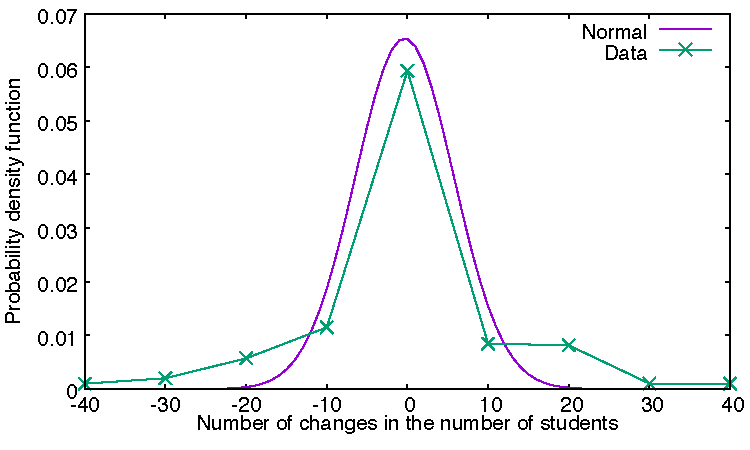
\includegraphics{perturbationsRoom.pdf}}
    \caption{}
    \label{fig:normalDistStu}
\end{subfigure}
\begin{subfigure}{.5\textwidth}\resizebox{\textwidth}{!}{
    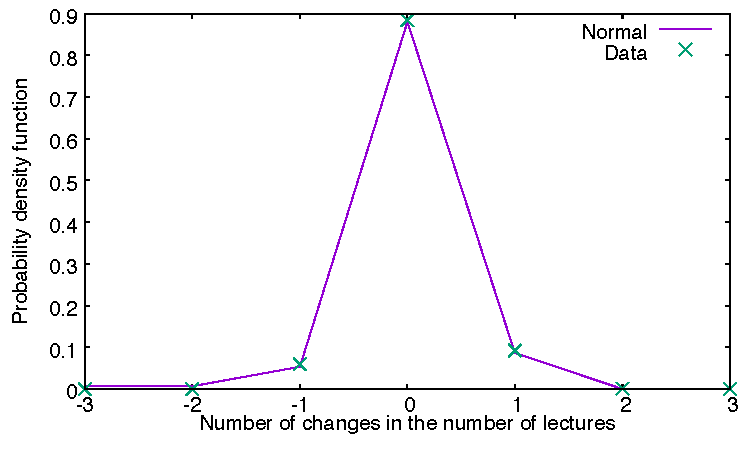
\includegraphics{perturbationsShift.pdf}}
    \caption{}
    \label{fig:normalDistShift}
\end{subfigure}
\captionof{figure}{Normal distribution that best fits the data sets of fluctuations in the (a) students enrollments (with mean of -0.3 and standard deviation of 6), and (b) the number of lectures (with mean of 0.04 and standard deviation of 0.45).}
\end{minipage}  
\end{figure*}

Table~\ref{tab:dataSet} shows a comparison between the data sets present in the literature. One can observe that the data set from \uni \ is considerably larger than the data sets from \gls{itc} and \gls{kul}. Furthermore, the data sets from \gls{itc} and \gls{kul} consider all lectures with the same length which can significantly simplify the encoding. Note that, the data set from \gls{kul} does not specify different capacities for each room. For this reason, the \textit{utilization} metric cannot be applied.

When analyzing the data set from \uni, one can see that room \textit{utilization} is higher than room \textit{frequency}. This can be easily explained by the need for lectures with overbooking~\citep{LEMOS2018100092} (\emph{i.e.} more students seated than actual seats). Note that, the \textbf{Taguspark} instances are going to be referenced from now on only by \textsc{FALL} and \textsc{SPRING}.



\subsection{Experimental Setup}

The solution was tested using the data sets from the courses taught in the Taguspark campus of \gls{ist}. We also have the current hand-made solution that can be used as starting point for the search algorithm. The values for $\alpha$ were previously obtained in~\cite{LEMOS2018100092} by optimizing this parameter.

The data is encoded with \gls{itc}-2019 XML format~\citep{itc-2019}. The code and data sets are available at \burlalt{https://github.com/ADDALemos/MPPTimetables/releases/tag/J.Scheduling19}{https://github.com/ADDALemos/MPPTimetables/releases/tag/J.Scheduling19}.
The data used to test the system was obtained through the FenixEdu\texttrademark system public API\footnote{\href{http://fenixedu.org/dev/api/}{http://fenixedu.org/dev/api/}} which is in use at \gls{ist}. 


The tests were run using the \textit{runsolver} tool~\citep{runsolver} with a time out of 600 seconds and a limit of 3 GB of memory. The tests were performed on a computer running Ubuntu 14, with 24 CPUs at 2.6 GHz and 64 Gb of RAM.

The program was implemented in C++, using the XML parser \textit{RAPIDXML}\footnote{\textit{RAPIDXML} is available from \url{http://rapidxml.sourceforge.net/manual.html}} to read the timetabling. The models were implemented using \textit{Gurobi}~\citep{gurobi}. The \textit{Gurobi} solver was run with parameters \textit{GRB\_IntParam\_Threads = 3} and \textit{GRB\_IntParam\_Presolve = 0} for best performance.




\subsection{Generating Disruptions}

To test our approach, we first analyzed the timetables from the last 5 years to identify which disruptions are the most common. These disruptions generally occur at the beginning of the new semester when a new timetable is generated. To compute the likelihood of a disruption to occur, we take into account the number of perturbations (Hamming distance) occurring from one year to another, over the total number of variables.  

\begin{table*}[!h]
	\caption{Results for \textsc{Boolean}, \textsc{Boolean'} and \textsc{mixed} models solving the university timetabling problem with warm-start, considering general (Gen.) and quadratic (Qua.) constraints. }
	\label{tab:static}
	\centering
	%\resizebox{\textwidth}{!}{%
		\begin{tabular}{l|c|c|c|c|c|c|c|c|}
			\cline{2-7}
			
			& \multicolumn{3}{c|}{\textsc{\textsc{FALL}}}   & \multicolumn{3}{c|}{\textsc{\textsc{SPRING}}} \\ \cline{2-7} 
			& \textsc{Boolean} & \textsc{Boolean'}     & \textsc{mixed}  & \textsc{Boolean}    & \textsc{Boolean'}    & \textsc{mixed}  \\ \hline
			%\multicolumn{1}{|c|}{Total CPU Time (s)} &  668.76                & 62.17      &   663.22        & 48.69      \\ \cline{1-5} 
			\multicolumn{1}{|l|}{CPU Time (s)} & Time Out & Time Out                  & 32.17      &    Time Out  &    Time Out            & 22.69      \\ \cline{1-7} 
			\multicolumn{1}{|l|}{Optimal}                        &   N/A &   N/A              &  Found     &    N/A &   N/A               &  Found     \\ \hline
			\multicolumn{1}{|l|}{\# Variables}                        &  5269200      &5280380  &  8487526              &  5255628     &5266548         &  1668712    \\ \hline
			\multicolumn{1}{|l|}{\# Gen. Constraints}                        &  5200000   & 5213975         & 2111238     & 5187000     & 5187000   &       1810312    \\ \hline
			\multicolumn{1}{|l|}{\# Qua. Constraints}                        &  5590     & 0          & 0     &  5460 & 0  &       0   \\ \hline
			
	\end{tabular}%}

\end{table*}


The average percentage of disruptions by type is shown in Table~\ref{tab:percentageD}. Note that \textit{time} and \textit{room assignment} represent the probability of a specific lecture to have a preference or a constraint in time or room assignment, respectively. We use these results to randomly generate the number of disruptions of the same type. The disruptions were randomly generated following a uniform distribution.



The information is shown in Table~\ref{tab:percentageD} is not enough for generating the full set of disruptions. In some cases, it is also necessary to correctly quantify the perturbations in a given lecture/course. This is the case of two specific disruptions: \textit{modify enrollments} and \textit{modify number of lectures}.

 For example, when modifying enrollments we need to decide in which lectures the number of students changes (based on the value from Table~\ref{tab:percentageD}) and the actual number to increase/decrease. One could analyze the changes and uniformly select one of these values since these values are not equiprobable. Therefore, we used the Microsoft Excel Solver~\citep{DBLP:journals/interfaces/FylstraLWW98} to estimate the parameters of a normal distribution that would best fit our data sets. Figure~\ref{fig:normalDistStu} shows the comparison between the closest-fit normal distribution and our data set.

 The same process can be applied to find the correct distribution for the disruption \textit{modify number of lectures}. Figure~\ref{fig:normalDistShift} shows the comparison between the closest-fit normal distribution and our data set.
 
\subsection{Computational Results}


\subsubsection{University Timetabling Problem} 


In a first approach, we compare the performance of the two different models (proposed in Section 4) when solving the original version of the problem, \emph{i.e.} before disruptions occur. Naturally, we considered the COM as the optimization criteria.  To improve performance, we apply a warm-start procedure using the hand-made solution. Note that, despite the fact the academic services use COM as the optimization criteria, the hand-made solution is feasible but not optimal. We also tested using greedy heuristics (the extension from our work \citep{LEMOS2018100092}). However, they are worse in terms of quality and similar in terms of CPU time. Therefore, we do not show the result.

Table~\ref{tab:static} shows the results for the different models (\textsc{Boolean}, \textsc{Boolean'} and \textsc{mixed}) when solving the university timetabling problem with warm-start. Observe that the \textsc{Boolean} model requires both general and quadratic constraints. The linearized version of the \textsc{Boolean} model only requires general constraints. However, it adds two new auxiliary variables for each quadratic constraints. The \textsc{Boolean'} model also adds two and half more constraints for each new variable. There is no clear advantage in the \textsc{Boolean} model versus \textsc{Boolean'} model with this time limit.  The \textsc{mixed} model requires fewer constraints and variables. In terms of CPU time, the \textsc{Boolean} model is not able to find an optimal solution within the 600 seconds limit. 


It is possible to reduce the size of the problem by reducing the number of students since not all students affect the solution. In this case, the students are used to identify the curricular path. It is natural that groups of students attend the same lectures. Therefore, one does not need to generate constraints for all students. The constraints can be generated only for \textit{distinct} students. In the data sets, around 15\% of all students attend exactly the same lectures. This number is relatively small but allows us to reduce the total number of constraints by 10\% on average for each instance. 

To study the impact of the warm-start strategy in the performance, we run the tests with and without this strategy for the \textsc{mixed} model. The results from \textsc{\textsc{FALL}} and \textsc{\textsc{SPRING}} improve from 1822.57 and 1726.21 to 32.17 and 22.69, respectively.  The version with warm-start is two orders of magnitude faster. The hand-made solution, despite not being optimal, is shown to be a good starting point. 



\subsubsection{Minimal Perturbation Problem}


\begin{table*}[!t]
\caption{Results for the most common disruptions using the \textsc{mixed} model. TO stands for time out, $\delta_{HD}$ measures the number of perturbations, $\delta_{WHD}$ measures the number of students affected by the perturbations and $\delta_{COM}$ measure the change in the number of gaps in the student’s timetable.}
\label{tab:recovery}
\centering
%\resizebox{\textwidth}{!}{%
\begin{tabular}{cl|c|c|c|c|c|c|}
\cline{3-8}
                                           &                   & \multicolumn{2}{c|}{\textit{Modify Enrollments}}& \multicolumn{2}{c|}{\textit{Invalid  Time}}& \multicolumn{2}{c|}{\textit{Invalid  Room}} \\ \hline
\multicolumn{1}{|c|}{Opt.}         &                   & \textsc{FALL}                &  \textsc{SPRING}   & \textsc{FALL}                &  \textsc{SPRING}    & \textsc{FALL}                &  \textsc{SPRING}      \\ \hline
\multicolumn{1}{|c|}{\multirow{7}{*}{COM}} & AVG.  Time (s)  & 46.2 & 20.65          & TO &TO       &73.36 &60.52                \\ \cline{2-8} 
\multicolumn{1}{|c|}{}                     & Median Time (s)   & 46.23 & 20.16     & TO &TO     & 72.34 &  59.95                      \\ \cline{2-8} 
\multicolumn{1}{|c|}{}                     & AVG.  $\delta_{COM}$ & -1 & -1.5       & \multicolumn{2}{c|}{N/A}     & 0.5&        0           \\ \cline{2-8} 
\multicolumn{1}{|c|}{}                     & COM \% Optimal    & 100                 &    100  &\multicolumn{2}{c|}{N/A}   &80 & 90           \\ \cline{2-8} 
\multicolumn{1}{|c|}{}                     & AVG.  $\delta_{HD}$ &     510         &   399      & \multicolumn{2}{c|}{N/A}   & 372&   340   \\ \cline{2-8} 
\multicolumn{1}{|c|}{}                     & AVG. $\delta_{WHD}$ &27303.9& 27287.1   & \multicolumn{2}{c|}{N/A}                 & 27000&   27602.5         \\ \cline{2-8}
\multicolumn{1}{|c|}{}                     & \% of Feasible Solution & 100 & 100   &\multicolumn{2}{c|}{N/A}               & 80&   90            \\ \hline

\multicolumn{1}{|c|}{\multirow{7}{*}{HD}} & AVG.  Time (s)  &   40.79 &        42.91   & TO & TO           & 74.45& 54.37           \\ \cline{2-8} 
\multicolumn{1}{|c|}{}                     & Median Time (s)   &  44 &   42.99         &TO &TO                  & 75& 51.9     \\ \cline{2-8} 
\multicolumn{1}{|c|}{}                     & AVG.  $\delta_{COM}$ &    0                 & 0   & \multicolumn{2}{c|}{N/A}              & 4.4&  0.87    \\ \cline{2-8} 
\multicolumn{1}{|c|}{}                     & AVG. $\delta_{HD}$ &   489 &  380        & \multicolumn{2}{c|}{N/A}                          & 300 &  309.75  \\ \cline{2-8} 
\multicolumn{1}{|c|}{}                     & HD \% Optimal    &        100             &         100   & \multicolumn{2}{c|}{N/A}     & 80 &  90      \\ \cline{2-8} 
\multicolumn{1}{|c|}{}                     & AVG. $\delta_{WHD}$ &   26803.5 & 26990.2      & \multicolumn{2}{c|}{N/A}                      &26660.83 & 27334.7         \\ \cline{2-8}
\multicolumn{1}{|c|}{}                     & \% of Feasible Solution & 100 & 100   & \multicolumn{2}{c|}{N/A}                    &80 &   90         \\ \hline

\multicolumn{1}{|c|}{\multirow{7}{*}{WHD}} & AVG.  Time (s)  &  39.97   &   43.6     & TO & TO & 69.17&                       60.28 \\ \cline{2-8} 
\multicolumn{1}{|c|}{}                     & Median Time (s)   &  44 & 43.99         & TO & TO      & 68.15&                    62.95  \\ \cline{2-8} 
\multicolumn{1}{|c|}{}                     & AVG.  $\delta_{COM}$ &       0              &      0   & \multicolumn{2}{c|}{N/A}     & 4.2&           0.6  \\ \cline{2-8} 
\multicolumn{1}{|c|}{}                     & AVG. $\delta_{HD}$ &  508 &   399    & \multicolumn{2}{c|}{N/A}                           & 490&        489 \\ \cline{2-8} 
\multicolumn{1}{|c|}{}                     & AVG. $\delta_{WHD}$ &   25908.5 & 26512.9   & \multicolumn{2}{c|}{N/A}                        &  26442     & 27468.12      \\ \cline{2-8} 
\multicolumn{1}{|c|}{}                     & WHD \% Optimal    &      100               &    100   & \multicolumn{2}{c|}{N/A}          &80 &     90  \\ \cline{2-8}
\multicolumn{1}{|c|}{}                     & \% of Feasible Solution & 100 & 100   & \multicolumn{2}{c|}{N/A}                    &80 &   90           \\ \hline

\end{tabular}%}
\end{table*}


The models proposed in this paper were also tested in the presence of disruptions. For each disruption type, 50 different instances were created. In this paper, we only show the results for the most relevant disruptions (\emph{i.e.} the disruptions that are likely to occur). The instances were generated based on the data analyzes explained above. We tested the models using all the disruptions found on the original data (see Table~\ref{tab:percentageD}). In this section, we discuss the most relevant disruptions.

Once again and as expected, the \textsc{mixed} model outperforms the \textsc{Boolean} model. For this reason, only the results for the \textsc{mixed} model are shown in Table~\ref{tab:recovery}. In order to improve performance, the warm-start strategy was modified to only add a partial solution (the variables affected by the disruption are not added).

The \textsc{\textsc{SPRING}} instance is easier to solve since it has a smaller number of lectures to assign. This fact can be explained by the organization of the curricular plans. 

\begin{table*}[!t]
	\centering
	\caption{Incremental approach to recover after disruptions of the type \textit{invalid time}. $\delta_{HD}$ measures the number of perturbations, $\delta_{WHD}$ measures the number of students affected by the perturbations and $\delta_{COM}$ measure the change in the number of gaps in the student’s timetable.}
	\label{tab:ite}
	\begin{tabular}{l|c|c|c|c|}
		\cline{2-5}
		& \multicolumn{2}{c|}{\textsc{FALL}} & \multicolumn{2}{c|}{\textsc{SPRING}} \\ \cline{2-5} 
		& Stage 1     & Stage 2     & Stage 1      & Stage 2      \\ \hline
		\multicolumn{1}{|c|}{Avg Time (s)}                & 239.02 & 68.67 & 210.68      & 58.4         \\ \hline
		\multicolumn{1}{|c|}{Median Time (s)}                 & 282         & 68          & 231.24       & 58           \\ \hline
		\multicolumn{1}{|c|}{Avg $\delta_{COM}$ }                     & 2           & 2           & 1            & 1            \\ \hline
		\multicolumn{1}{|c|}{AVG $\delta_{HD}$}                     & 416.67 & 416.67 & 400.34  & 400.34  \\ \hline
		\multicolumn{1}{|c|}{AVG $\delta_{WHD}$}                     & 26726.34 & 26726.34 & 27473.34  & 27473.34  \\ \hline
		\multicolumn{1}{|c|}{\% Feasible Solution} & \multicolumn{2}{c|}{85}   & \multicolumn{2}{c|}{90}     \\ \hline
	\end{tabular}
\end{table*}


When analyzing the performance one can see that the \textit{modify enrollment} disruption instances are the easiest to be solved. This can be explained by the fact the disruption adds, in general, only a small number of students. The use of slack in room capacities also contributes to better performance. This is the only disruption that is able to improve the value of the COM (when optimizing this criterion). This disruption also allows reducing the number of students enrolled. \textit{Modify enrollments} is the only disruption to have all instances with a feasible solution. The HD and WHD optimization criteria reduce the number of perturbations and the number of students affected while not improving the COM. For this disruption, the value of COM stays equal to the one found in the original solution.

The disruptions \textit{invalid time assignment} and \textit{invalid room assignment} cannot lead to a solution with an improved optimization value, given that these disruptions only add new constraints to the problem. The results show that the quality of the solution gets worse with these disruptions. Note that these disruptions may cause the instance to be infeasible. For all instances with feasible solutions, our approach finds optimal solutions. The \textit{invalid time assignment} disruption is the only one to reach the time limit before finding a solution. 

Globally, one can see that optimizing using COM causes more perturbations in the solution and affects more students. This result confirms the results obtained by \cite{LINDAHL2019}, where it is said that performing more perturbations can improve the quality of the solution. Optimizing based the WHD criteria also causes more perturbations but reduces the number of students affected by the change.  



\subsubsection{Incremental Approach for Recovery after Disruption}



The simple recovery process takes too long for the \textit{invalid time assignment} disruption. Therefore, we propose an incremental approach to reduce the search space by splitting the problem into two stages.  A disruption of the type \textit{invalid time assignment} clearly causes a change in the time slots of the lecture. However, it may not be necessary to modify the room assignment. For this reason, we divide the problem into: (i) the problem of assignment of lectures to rooms and (ii) the whole problem. The first stage has to deal with all the constraints relating to time slots, where one has to consider a solution to the problem of assigning rooms to lectures. In this case, the original solution for this sub-problem is added to the model as static. The second stage applies a warm-start with the results of the first stage, possibly improving its quality. This division does not exclude possible solutions since the second stage includes the whole problem again. This decomposition can be changed (\emph{i.e.} start with the problem of assigning lectures to rooms) depending on the disruption since we know beforehand which part of the problem must change. 

Naturally, the proposed decomposition does not provide any guarantees about optimality at the end of the first stage. Nevertheless, this decomposition ensures that a feasible solution to the first stage is a feasible solution to the whole problem. Conversely, one cannot conclude anything about the infeasibility of the instance based on the result from the first stage.  

Table~\ref{tab:ite} shows the results for the \textit{invalid time assignment} disruption, where one can see that the incremental process is much faster. In this case, the second stage does not improve the quality of the solution. In other words, the first stage not only found a feasible solution but also found an optimal solution to the complete problem. % However, only at the end of the second stage, one can prove that the solution is indeed optimal.





\section{Conclusion and Future Work}\label{sec:con}

This paper discusses the problem of solving university timetabling problems after the occurrence of disruptions, namely, the methods to solve the \gls{mpp} for real-world university timetabling problems.

The two integer programming models proposed can find the \textit{closest} new feasible solution for most common university timetabling disruption scenarios. Our approaches were successfully evaluated with data sets from \uni. To correctly test the performance of the methods, we randomly generated disruptions with the probability learned from the history of the last five years of timetables.
The models were tested using different optimization criteria, including the optimization criteria applied by the academic offices at \uni.

To improve the performance, we propose an incremental algorithm that divides the problem into two stages: the problem of assignment of lectures to rooms and the whole problem.
The incremental algorithm can reduce the size and execution time without losing quality.
Moreover, the experimental results also show that using warm-start techniques in this type of problems provides a significant advantage.
We warm-start the algorithm with a partial feasible solution extracted from the solution of the previous year.

As future work, we propose to extend this method in order to exploit the incremental nature of MPP. This way, every time a new disruption arises, {\em only} another step in the incremental integer programming algorithm would be required. The usage of incremental algorithms would reduce CPU time by avoiding the repetition of redundant steps when searching for a new feasible solution.


%\section*{Acknowledgements}
%\footnotesize{}



\newacronym{kul}{KUL}{Katholieke Universiteit Leuven}
\newacronym{asp}{ASP}{Answer Set Programming}
\newacronym{mpp}{MPP}{Minimal Perturbation Problem}
\newacronym{ilp}{ILP}{Integer Linear Programming}
\newacronym{ist}{IST}{Instituto Superior T\'ecnico}
\newacronym{cp}{CP}{Constraint Programming}
\newacronym{itc}{ITC}{International Timetabling Competition}



\bibliographystyle{spbasic} \bibliography{cite}



\end{document}
